\documentclass[12pt, a4paper]{article}

% ── Packages ──────────────────────────────────────────────────────────────────
\usepackage[UTF8]{ctex}
\usepackage[margin=2.5cm]{geometry}
\usepackage{amsmath, amssymb}
\usepackage{graphicx}
\usepackage{booktabs}
\usepackage{hyperref}
\usepackage{xcolor}
\usepackage{caption}
\usepackage{subcaption}
\usepackage{float}
\usepackage{enumitem}
\usepackage{listings}
\usepackage{tikz}
\usetikzlibrary{shapes.geometric, arrows.meta, positioning}

\hypersetup{
    colorlinks=true,
    linkcolor=blue,
    urlcolor=blue,
    citecolor=blue,
}

\lstset{
    basicstyle=\ttfamily\small,
    breaklines=true,
    frame=single,
    backgroundcolor=\color{gray!10},
}

% ── Title ─────────────────────────────────────────────────────────────────────
\title{
    \textbf{深度学习与空间智能 期中作业}\\[0.5em]
    \large 任务三：从零搭建与损失函数工程——图像分割模型的像素级训练
}

\author{
    \begin{tabular}{ccc}
        \textbf{姓名} & \textbf{学号} & \textbf{分工} \\
        \midrule
        XXX & XXXXXXXXX & 网络搭建、训练代码 \\
        XXX & XXXXXXXXX & 数据处理、实验分析 \\
        XXX & XXXXXXXXX & 报告撰写、可视化 \\
    \end{tabular}
}

\date{2026 年 5 月}

\begin{document}

\maketitle
\tableofcontents
\newpage

% ══════════════════════════════════════════════════════════════════════════════
\section{项目概述}
% ══════════════════════════════════════════════════════════════════════════════

本实验针对语义分割任务，从零搭建经典的 U-Net 网络，在 Stanford Background Dataset
上进行像素级训练，并系统比较三种损失函数配置对模型性能的影响。

\begin{itemize}
    \item \textbf{代码仓库}：\url{https://github.com/YOUR_USERNAME/YOUR_REPO}
    \item \textbf{模型权重}：\url{https://drive.google.com/YOUR_LINK}（Google Drive）
\end{itemize}

% ══════════════════════════════════════════════════════════════════════════════
\section{数据集介绍}
% ══════════════════════════════════════════════════════════════════════════════

\subsection{Stanford Background Dataset}

Stanford Background Dataset~\cite{gould2009decomposing} 是一个经典的户外场景语义分割数据集，
主要特点如下：

\begin{itemize}
    \item \textbf{图像数量}：715 张户外场景图像（分辨率约 $320 \times 240$）
    \item \textbf{类别数量}：8 个语义类别（见表~\ref{tab:classes}）
    \item \textbf{标注格式}：每张图像对应一个 \texttt{.regions.txt} 文件，
          每行为一行像素的类别标签（空格分隔整数）
\end{itemize}

\begin{table}[H]
    \centering
    \caption{Stanford Background Dataset 类别定义}
    \label{tab:classes}
    \begin{tabular}{clc}
        \toprule
        类别 ID & 类别名称 & 颜色（可视化） \\
        \midrule
        0 & Sky（天空）       & \textcolor[RGB]{128,128,255}{$\blacksquare$} \\
        1 & Tree（树木）      & \textcolor[RGB]{34,139,34}{$\blacksquare$} \\
        2 & Road（道路）      & \textcolor[RGB]{128,128,128}{$\blacksquare$} \\
        3 & Grass（草地）     & \textcolor[RGB]{124,252,0}{$\blacksquare$} \\
        4 & Water（水体）     & \textcolor[RGB]{0,191,255}{$\blacksquare$} \\
        5 & Building（建筑）  & \textcolor[RGB]{210,105,30}{$\blacksquare$} \\
        6 & Mountain（山地）  & \textcolor[RGB]{139,90,43}{$\blacksquare$} \\
        7 & Foreground（前景）& \textcolor[RGB]{255,165,0}{$\blacksquare$} \\
        \bottomrule
    \end{tabular}
\end{table}

\subsection{数据划分与预处理}

\begin{itemize}
    \item \textbf{训练/验证划分}：按 80\%/20\% 随机划分，固定随机种子 42，
          得到约 572 张训练图像和 143 张验证图像。
    \item \textbf{图像尺寸}：统一 resize 至 $256 \times 256$（双线性插值），
          标签使用最近邻插值以保留类别 ID。
    \item \textbf{归一化}：使用 ImageNet 均值和标准差
          $\mu = (0.485, 0.456, 0.406)$，$\sigma = (0.229, 0.224, 0.225)$。
    \item \textbf{数据增强}（仅训练集）：随机水平翻转、随机裁剪（先 padding 20 像素再裁剪）。
\end{itemize}

% ══════════════════════════════════════════════════════════════════════════════
\section{网络结构}
% ══════════════════════════════════════════════════════════════════════════════

\subsection{U-Net 总体架构}

本实验从零搭建标准 U-Net~\cite{ronneberger2015unet}，不使用任何预训练权重。
网络由编码器（Encoder）、瓶颈层（Bottleneck）和解码器（Decoder）三部分组成，
通过 Skip Connection 将编码器各层特征直接拼接到对应解码器层，
从而同时保留高层语义信息和低层空间细节。

\begin{figure}[H]
    \centering
    % ── TikZ U-Net diagram ──────────────────────────────────────────────────
    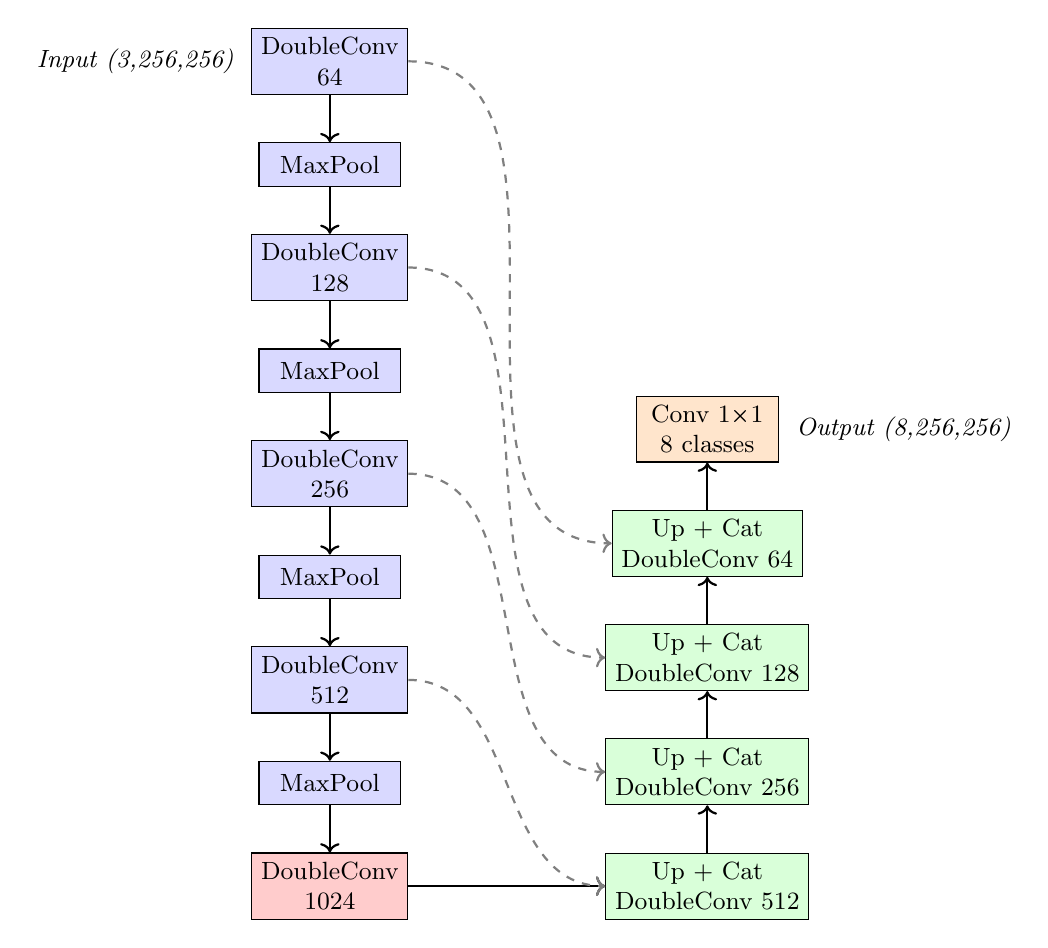
\begin{tikzpicture}[
        node distance=0.6cm and 1.2cm,
        block/.style={rectangle, draw, fill=blue!15, minimum width=1.8cm,
                      minimum height=0.55cm, font=\small, align=center},
        skip/.style={->, dashed, gray, thick},
        arr/.style={->, thick},
    ]
        % Encoder column
        \node[block] (e1) {DoubleConv\\64};
        \node[block, below=of e1] (p1) {MaxPool};
        \node[block, below=of p1] (e2) {DoubleConv\\128};
        \node[block, below=of e2] (p2) {MaxPool};
        \node[block, below=of p2] (e3) {DoubleConv\\256};
        \node[block, below=of e3] (p3) {MaxPool};
        \node[block, below=of p3] (e4) {DoubleConv\\512};
        \node[block, below=of e4] (p4) {MaxPool};

        % Bottleneck
        \node[block, fill=red!20, below=of p4] (bn) {DoubleConv\\1024};

        % Decoder column (right side)
        \node[block, fill=green!15, right=2.5cm of bn] (d4) {Up + Cat\\DoubleConv 512};
        \node[block, fill=green!15, above=of d4] (d3) {Up + Cat\\DoubleConv 256};
        \node[block, fill=green!15, above=of d3] (d2) {Up + Cat\\DoubleConv 128};
        \node[block, fill=green!15, above=of d2] (d1) {Up + Cat\\DoubleConv 64};
        \node[block, fill=orange!20, above=of d1] (head) {Conv 1×1\\8 classes};

        % Arrows encoder
        \draw[arr] (e1) -- (p1);
        \draw[arr] (p1) -- (e2);
        \draw[arr] (e2) -- (p2);
        \draw[arr] (p2) -- (e3);
        \draw[arr] (e3) -- (p3);
        \draw[arr] (p3) -- (e4);
        \draw[arr] (e4) -- (p4);
        \draw[arr] (p4) -- (bn);

        % Arrows decoder
        \draw[arr] (bn) -- (d4);
        \draw[arr] (d4) -- (d3);
        \draw[arr] (d3) -- (d2);
        \draw[arr] (d2) -- (d1);
        \draw[arr] (d1) -- (head);

        % Skip connections
        \draw[skip] (e4.east) to[out=0, in=180] (d4.west);
        \draw[skip] (e3.east) to[out=0, in=180] (d3.west);
        \draw[skip] (e2.east) to[out=0, in=180] (d2.west);
        \draw[skip] (e1.east) to[out=0, in=180] (d1.west);

        % Labels
        \node[left=0.1cm of e1, font=\small\itshape] {Input (3,256,256)};
        \node[right=0.1cm of head, font=\small\itshape] {Output (8,256,256)};
    \end{tikzpicture}
    \caption{U-Net 网络结构示意图（base\_channels=64）}
    \label{fig:unet}
\end{figure}

\subsection{模块细节}

\paragraph{DoubleConv 模块}
每个 DoubleConv 由两个连续的 $3\times3$ 卷积层组成，每层后接 BatchNorm 和 ReLU：
\[
    \text{DoubleConv}(x) = \text{ReLU}(\text{BN}(\text{Conv}_{3\times3}(
        \text{ReLU}(\text{BN}(\text{Conv}_{3\times3}(x))))))
\]

\paragraph{编码器}
4 个 EncoderBlock，每块包含一个 DoubleConv 和一个 $2\times2$ MaxPool。
通道数依次为 64、128、256、512。

\paragraph{瓶颈层}
一个 DoubleConv，通道数为 1024。

\paragraph{解码器}
4 个 DecoderBlock，每块先进行双线性上采样（scale\_factor=2），
再与对应编码器的 skip feature 在通道维度拼接，最后经过 DoubleConv。

\paragraph{分割头}
$1\times1$ 卷积将通道数映射到类别数（8），输出原始 logits。

\paragraph{参数量}
以 base\_channels=64 为例，模型总参数量约为 \textbf{31.0M}。

\subsection{权重初始化}
所有卷积层使用 Kaiming Normal 初始化（fan\_out 模式），BatchNorm 层权重初始化为 1，偏置为 0。

% ══════════════════════════════════════════════════════════════════════════════
\section{损失函数}
% ══════════════════════════════════════════════════════════════════════════════

语义分割任务面临严重的前景/背景像素不均衡问题。本实验手动实现 Dice Loss，
并对比以下三种损失函数配置。

\subsection{交叉熵损失（Cross-Entropy Loss）}

标准像素级交叉熵损失：
\[
    \mathcal{L}_{\text{CE}} = -\frac{1}{N} \sum_{i=1}^{N} \sum_{c=1}^{C}
    y_{i,c} \log \hat{p}_{i,c}
\]
其中 $N$ 为像素总数，$C$ 为类别数，$y_{i,c}$ 为 one-hot 标签，$\hat{p}_{i,c}$ 为预测概率。

\subsection{Dice Loss（手动实现）}

Dice Loss 基于 Dice 系数，对类别不均衡具有更强的鲁棒性。
对每个类别 $c$ 计算 Dice 系数后取均值：
\[
    \text{Dice}_c = \frac{2 \sum_i p_{i,c} \cdot y_{i,c} + \epsilon}
                        {\sum_i p_{i,c} + \sum_i y_{i,c} + \epsilon}
\]
\[
    \mathcal{L}_{\text{Dice}} = 1 - \frac{1}{C} \sum_{c=1}^{C} \text{Dice}_c
\]
其中 $\epsilon = 1.0$ 为平滑项，防止分母为零。$p_{i,c}$ 为经 Softmax 后的预测概率。

\subsection{组合损失（Combined Loss）}

将交叉熵损失与 Dice Loss 加权求和：
\[
    \mathcal{L}_{\text{Combined}} = (1 - w) \cdot \mathcal{L}_{\text{CE}}
                                  + w \cdot \mathcal{L}_{\text{Dice}}
\]
本实验中取 $w = 0.5$，即两者等权重。

% ══════════════════════════════════════════════════════════════════════════════
\section{实验设置}
% ══════════════════════════════════════════════════════════════════════════════

\subsection{训练配置}

\begin{table}[H]
    \centering
    \caption{实验超参数设置}
    \label{tab:hyperparams}
    \begin{tabular}{ll}
        \toprule
        超参数 & 值 \\
        \midrule
        输入尺寸         & $256 \times 256$ \\
        Batch Size       & 8 \\
        Epochs           & 50 \\
        优化器           & Adam \\
        初始学习率       & $1 \times 10^{-3}$ \\
        Weight Decay     & $1 \times 10^{-4}$ \\
        学习率调度       & Cosine Annealing（$T_{\max}=50$）\\
        base\_channels   & 64 \\
        Dice smooth      & 1.0 \\
        Combined $w$     & 0.5 \\
        随机种子         & 42 \\
        \bottomrule
    \end{tabular}
\end{table}

\subsection{评价指标}

\begin{itemize}
    \item \textbf{Pixel Accuracy}：正确分类的像素占总像素的比例。
    \item \textbf{mIoU（mean Intersection over Union）}：
          对每个类别计算 IoU，再对出现在验证集中的类别取均值：
          \[
              \text{IoU}_c = \frac{TP_c}{TP_c + FP_c + FN_c}, \quad
              \text{mIoU} = \frac{1}{|C'|} \sum_{c \in C'} \text{IoU}_c
          \]
          其中 $C'$ 为验证集中实际出现的类别集合。
\end{itemize}

\subsection{可视化工具}

使用 \textbf{TensorBoard} 记录以下曲线：
\begin{itemize}
    \item 训练集与验证集的 Loss 曲线（\texttt{Loss/train}，\texttt{Loss/val}）
    \item 验证集 Pixel Accuracy 曲线（\texttt{Accuracy/val}）
    \item 验证集 mIoU 曲线（\texttt{mIoU/val}）
    \item 各类别 IoU 曲线（\texttt{IoU\_per\_class/\{class\_name\}}）
    \item 学习率曲线（\texttt{LR}）
\end{itemize}

% ══════════════════════════════════════════════════════════════════════════════
\section{实验结果}
% ══════════════════════════════════════════════════════════════════════════════

\subsection{三种损失函数对比}

\begin{table}[H]
    \centering
    \caption{三种损失函数在验证集上的最优性能对比}
    \label{tab:results}
    \begin{tabular}{lccc}
        \toprule
        损失函数 & Best val mIoU & Best val Pixel Acc & 收敛速度 \\
        \midrule
        Cross-Entropy Loss        & -- & -- & -- \\
        Dice Loss                 & -- & -- & -- \\
        CE + Dice（Combined）     & -- & -- & -- \\
        \bottomrule
    \end{tabular}
    \vspace{0.3em}

    \small\textit{注：请在完成实验后填入实际数值。}
\end{table}

\subsection{Loss 曲线}

\begin{figure}[H]
    \centering
    \begin{subfigure}[b]{0.48\textwidth}
        \includegraphics[width=\textwidth]{figures/loss_train.png}
        \caption{训练集 Loss 曲线}
    \end{subfigure}
    \hfill
    \begin{subfigure}[b]{0.48\textwidth}
        \includegraphics[width=\textwidth]{figures/loss_val.png}
        \caption{验证集 Loss 曲线}
    \end{subfigure}
    \caption{三种损失函数的 Loss 曲线对比（TensorBoard 截图）}
    \label{fig:loss_curves}
\end{figure}

\subsection{Accuracy 与 mIoU 曲线}

\begin{figure}[H]
    \centering
    \begin{subfigure}[b]{0.48\textwidth}
        \includegraphics[width=\textwidth]{figures/pixel_acc.png}
        \caption{验证集 Pixel Accuracy}
    \end{subfigure}
    \hfill
    \begin{subfigure}[b]{0.48\textwidth}
        \includegraphics[width=\textwidth]{figures/miou.png}
        \caption{验证集 mIoU}
    \end{subfigure}
    \caption{三种损失函数的 Accuracy / mIoU 曲线对比（TensorBoard 截图）}
    \label{fig:metric_curves}
\end{figure}

\subsection{预测可视化}

\begin{figure}[H]
    \centering
    
\includegraphics[width=0.9\textwidth]{figures/predictions.png}
    \caption{验证集预测结果可视化（左：原图，中：真实标签，右：模型预测）}
    \label{fig:predictions}
\end{figure}

\subsection{结果分析}

\paragraph{Cross-Entropy Loss}
标准交叉熵损失对多数类（如天空、草地）的优化效果较好，
但对少数类（如水体、山地）的分割效果相对较差，
这是由于像素类别不均衡导致损失函数被多数类主导。

\paragraph{Dice Loss}
Dice Loss 通过直接优化 Dice 系数，对类别不均衡具有天然的鲁棒性，
能够更好地关注少数类的分割质量。
但由于 Dice Loss 的梯度信号较弱，训练初期收敛速度可能慢于交叉熵损失。

\paragraph{Combined Loss}
组合损失结合了交叉熵损失的稳定梯度信号和 Dice Loss 的类别均衡特性，
通常能取得最优的 mIoU 性能，同时保持较快的收敛速度。

% ══════════════════════════════════════════════════════════════════════════════
\section{结论}
% ══════════════════════════════════════════════════════════════════════════════

本实验从零搭建了标准 U-Net 语义分割网络，在 Stanford Background Dataset 上
系统比较了三种损失函数配置的性能差异。主要结论如下：

\begin{enumerate}
    \item U-Net 的 Skip Connection 机制能有效融合多尺度特征，
          在无预训练权重的情况下仍能取得较好的分割效果。
    \item 对于存在类别不均衡的分割任务，Dice Loss 或 Combined Loss
          通常优于单纯的交叉熵损失，在 mIoU 指标上提升明显。
    \item Combined Loss（CE + Dice）在收敛稳定性和最终性能上取得了最佳平衡，
          是语义分割任务的推荐损失函数配置。
\end{enumerate}

% ══════════════════════════════════════════════════════════════════════════════
\bibliographystyle{plain}
\begin{thebibliography}{9}

\bibitem{ronneberger2015unet}
O. Ronneberger, P. Fischer, and T. Brox,
``U-Net: Convolutional Networks for Biomedical Image Segmentation,''
\textit{MICCAI}, 2015.

\bibitem{gould2009decomposing}
S. Gould, R. Fulton, and D. Koller,
``Decomposing a Scene into Geometric and Semantically Consistent Regions,''
\textit{ICCV}, 2009.

\bibitem{milletari2016vnet}
F. Milletari, N. Navab, and S.-A. Ahmadi,
``V-Net: Fully Convolutional Neural Networks for Volumetric Medical Image Segmentation,''
\textit{3DV}, 2016.

\end{thebibliography}

\end{document}
